\section{Background Theory}

\subsection{Software used}
\subsubsection{OpenWRT router software}
OpenWRT is an open-source linux distrubution for embedded devices, typically wireless routers.

\subsubsection{SoftEther VPN Bridge}
\label{sec:comms_theory_vpn} % This needs to stay - we refer to here from web. ok
SoftEther VPN Bridge is software that allows you to cascade-connect to a Virtual Hub of a SoftEther VPN Server operating at a remote location and create a Layer-2 bridge connection between that VPN connection and a physical network adapter on a computer running SoftEther VPN Bridge. SoftEther VPN Bridge is the ideal software for a computer connected to a remote base LAN when you want to connect the remote base LAN to a VPN configured with SoftEther VPN Server (namely, a Virtual Hub on a SoftEther VPN Server).

need a better explaination of how vpns work here with a diagram 

\subsection{Hardware used}
\subsubsection{Biquad Yagi Antenna}
The Biquad Yagi is a hybrid antenna based on the biquad antenna

\begin{figure}[!htb]
\begin{center}
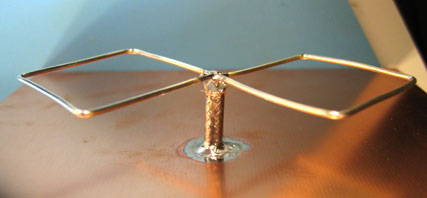
\includegraphics[width=15cm]{bi-quad_side.jpg}
\end{center}
\caption{Biquad Antenna}
\label{fig:biquad}
\end{figure}


and the Yagi-Uda antenna


\begin{figure}[!htb]
\begin{center}
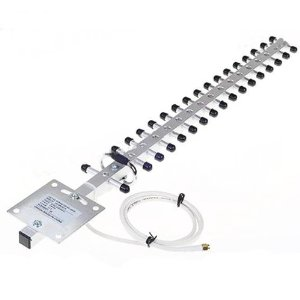
\includegraphics[width=10cm]{yagi.jpg}
\end{center}
\caption{Yagi-Uda Antenna}
\label{fig:yagi}
\end{figure}


